
\graphicspath{ {/home/ranguy/main/projects/Doom64Online/LATEX_REPORT_TEMPLATE/Mini project report template/images/} }

\section{Introduction}
\label{chap:introduction}

This report delves into the analysis of a complex and intriguing LAN-based multiplayer adaptation of the classic game Doom 64, named "Doom64 Online." The project has been selected for its intricate blend of retro gaming elements and advanced networking concepts. This fusion presents an opportunity to explore and understand the challenges and intricacies involved in modernizing a classic game for contemporary networked multiplayer environments.

\subsection{Features of Doom64 Online}

In "Doom64 Online," we have adapted and implemented several core features from the original Doom 64, tailored to create an engaging LAN-based multiplayer experience. The key features implemented in our adaptation are:

\begin{itemize}
    \item \textbf{Multiplayer Interaction:} Players can see and interact with other players within the game environment, enhancing the multiplayer experience and fostering a sense of community and competition.
    \item \textbf{Shooting Mechanics:} A fundamental aspect of the game is the ability to engage in combat by shooting at other players, adding a competitive and interactive dimension to the gameplay.
    \item \textbf{Player Movement:} Players have the ability to navigate freely around the game environment, enabling exploration and strategic positioning during gameplay.
    \item \textbf{3D Visualized Environment:} The game offers a fully immersive 3D environment, meticulously designed to replicate the atmospheric and intricate level design of the original Doom 64.
\end{itemize}

These features are central to "Doom64 Online," offering players a modernized version of the classic game with enhanced networked multiplayer capabilities.

\subsection{Reason for Selection}

The decision to analyze this project is driven by the following:
\begin{itemize}
    \item \textbf{Technical Insights:} The use of Python and Pygame \cite{pygame} offers a unique opportunity to apply networking principles in a game development context, providing insights into real-time data transfer, concurrency handling, and network efficiency in multiplayer games.
    \item \textbf{Educational Value:} It serves as an educational tool for understanding the application of socket programming, UDP communication, and game loop management in a Python-based environment.
    \item \textbf{Personal Interest:} The choice is also influenced by a personal fascination with the technical aspects of game development and the unique challenges posed by networked multiplayer game programming.
    \item \textbf{Multiplayer Game Development:} The project offers an opportunity to learn how AAA multiplayer games are implemented at a lower level by building it from scratch, instead of merely following pre-established frameworks or methodologies. This approach allows for a deeper understanding of the underlying mechanics and challenges involved in high-end game development.
\end{itemize}

\subsection{Analysis Focus and Hypotheses}

The analysis revolves around several key areas:

\begin{itemize}
    \item \textbf{Networking Implementation:} How does the project handle real-time communication and data synchronization between the server and multiple clients?
    \item \textbf{Concurrency Management:} How are multiple concurrent player interactions managed without compromising game performance?
    \item \textbf{Gameplay Integrity:} How does the networked environment affect gameplay, and what measures are in place to maintain game integrity and responsiveness?
\end{itemize}

The hypothesis is that the Doom64 Online project effectively utilizes Python's networking capabilities to create a seamless multiplayer experience, overcoming the challenges of latency and data consistency.



\subsection{Research questions/hypotheses}
\label{sec:question}

The following research questions and hypotheses are formulated to guide the analysis of the Doom64 Online project and will be pivotal in user evaluation:

\begin{enumerate}
    
    \item \textbf{Concurrency and Multiplayer Interaction:} How are concurrent actions from multiple players managed and synchronized by the server? Does the game maintain consistency in the shared game world across all clients?
    
    \item \textbf{Scalability of the Game Architecture:} Can the network architecture of Doom64 Online efficiently scale to accommodate an increasing number of players without degrading performance or gameplay experience?
    
    \item \textbf{Gameplay Mechanics and Network Dependence:} To what extent do the game's mechanics rely on network performance? Are there fallback mechanisms to handle network instability?
    
    \item \textbf{Implementation Challenges:} What are the primary challenges faced during the implementation of networked multiplayer features in Doom64 Online, and how were they addressed?
    
    \item \textbf{Comparison with AAA Game Standards:} How does the networking implementation in Doom64 Online compare with standard practices in AAA multiplayer games? Are there any noticeable differences in approaches to network management, data handling, and player synchronization?
    
\end{enumerate}
\section{Background}
\label{chap:background}


The challenge of efficient data sharing in multiplayer gaming environments is a well-explored domain, with numerous solutions proposed over the years. Fundamentally, this challenge revolves around the rapid and reliable transmission of game-related data such as player positions, health status, and various state variables. Two primary approaches have emerged as the most prevalent in addressing this problem: peer-to-peer (P2P) and client-server architectures.

In the peer-to-peer model, as detailed in existing literature \cite{peertopeer}, each player directly connects with other players, facilitating a decentralized exchange of data. While this approach enables direct data sharing among participants, it lacks a centralized validation mechanism, potentially leading to issues such as cheating and data inconsistency.

Conversely, the client-server model \cite{clientserver} centralizes data exchange, where all players connect to a dedicated server. This server acts as an authoritative source, validating and relaying data among players. This method enhances security and data integrity, as the server verifies all shared information before dissemination. However, its major drawback is the dependency on a single point of failure; server downtime directly impacts all connected players, rendering the game non-functional.

This project aims to delve into the intricacies of implementing a robust client-server communication system for a specific multiplayer game. We explore both UDP and TCP protocols to determine their suitability in different gaming scenarios, comparing their efficiency in handling real-time data exchange. Additionally, we evaluate various data packet formats, ranging from binary (like Pickle) to text-based (such as JSON), to ascertain the most effective method for data serialization and transmission.

To address concurrency, a critical aspect of multiplayer gaming, we investigate several programming constructs and system calls. These include traditional methods like os.fork, as well as more modern approaches such as the multithreading and multiprocessing libraries in Python. Each method is tested for its ability to handle simultaneous requests and data processing, ensuring that the game maintains consistent performance and responsiveness under varying load conditions.
% \newline
% \hrule
% \newline


\section{Data}
\label{chap:data}

The dataset for this project primarily revolves around the core assets and gameplay mechanics obtained from the open-source repository for a basic implementation of a DOOM-style game, accessible at \cite{doom-repo}. This foundational codebase serves as the starting point for the implementation of our networked multiplayer adaptation, "Doom64 Online."

\subsection{Data Preparation}
\label{sec:data preparation}

The adaptation of the base game into a multiplayer environment necessitated the development of a robust application layer from scratch. A critical aspect of this development was the design and implementation of custom communication message classes. These classes are instrumental in managing the data flow between the game clients and the server, ensuring efficient and reliable data exchange.

For data serialization and transmission, we opted for JSON, owing to its widespread use and ease of integration with Python. The message classes were designed to encapsulate various types of game-related information, such as player positions, game state updates, and login requests/responses. The following code snippet provides an overview of these classes:

\begin{lstlisting}[style=pythonstyle]





Code snippet for custom message classes

from settings import *
import json




class PacketClass:
    type = None
    msg = None
    def   init  (self,type=None,msg=None):
        self.type=type
        self.msg=msg

class LoginResMsg:
	x=0
	y=0
	id=None
	def   init  (self,x,y,id):
		self.x=x
		self.y=y
		self.id=id
	def getJson(self):
		return json.dumps(self.  dict  )

# this is an example implementation for one of the message class used for login
# (Note: For complete code, refer to the project repository)

\end{lstlisting}

These classes are a cornerstone in the architecture of Doom64 Online, facilitating the translation of game actions into network messages and vice versa. The JSON conversion capability integrated within these classes ensures a standardized format for data exchange, contributing to the overall consistency and reliability of the multiplayer experience.

\subsection{Significance of Data Preparation}
The design and implementation of these message classes were pivotal in achieving several project objectives:
\begin{itemize}
\item \textbf{Efficient Data Handling:} By using JSON for data serialization, the project benefits from a lightweight and easily parsable data format, crucial for real-time gaming scenarios.
\item \textbf{Scalability:} The modular nature of these classes allows for easy expansion and modification, essential for accommodating future enhancements or changes in game mechanics.
\item \textbf{Network Transparency:} Custom message classes provide a clear and structured way to handle various types of network communication, enhancing the maintainability and readability of the code.
\end{itemize}

In conclusion, the careful preparation and design of the data handling mechanisms in Doom64 Online play a critical role in ensuring the seamless operation and scalability of the game's multiplayer functionality.

% \section{Data}
% \label{chap:data}
% Briefly describe the dataset and the parameters that will be important for you in order to answer your questions/hypotheses. Indicate the source. If available online, providing a URL link helps the readers.

% \subsection{Data preparation}
% \label{sec:data}
% Describe what you did in order to use the data for analysis.





\section{Approach}
\label{chap:approach}

This section presents the approach adopted in the development of "Doom64 Online".

\subsection{L0: Design}
The project utilizes a server-client architecture for its communication system. The key features of this implementation include:

\begin{itemize}
    \item \textbf{Concurrent Server}: The server is equipped to handle multiple clients concurrently, aiming to provide low latency for each player.
    \item \textbf{Game State Management}: Server-side management ensures synchronization of game events across all connected clients, maintaining gameplay consistency.
    \item \textbf{Client Communication System}: Custom message classes are implemented for effective encoding and decoding of messages sent between the server and clients, tailored to the type of message transmitted over the network.
    \item \textbf{Server Finder}: To avoid the impracticality of manually entering the server's IP address on each client, a server finder feature is implemented for automatic detection of the server on the local network.
\end{itemize}


\textbf{L0 DIAGRAM:}
\newline 
\hfill \break
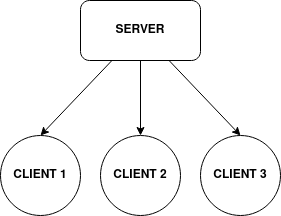
\includegraphics{L0}


\subsection{L1: Detailed Overview}
The primary communication components are consistent throughout all implementations of this project.

\subsubsection{Server}
The server comprises four fundamental components:
\begin{itemize}
    \item \textbf{Shared Memory Object}: Named GAME STATE, this component holds all player data, a list of game events, and other vital information to synchronize game events across players.
    \item \textbf{Main Listener Class}: This communication API establishes a connection listener, assigns unique ports to clients, and initiates a new thread for each connection, managing all client communications.
    \item \textbf{Client Communication Thread}: A dedicated thread for each client manages all communication with that client using a custom message class for encoding and decoding messages.
    \item \textbf{MultiCliCon Class}: This communication API facilitates interaction between the server thread and clients. It manages message processing, login requests, and responses.
\end{itemize}

\subsubsection{Client}
The client includes three base components:
\begin{itemize}
    \item \textbf{Main Connection Class}: This communication API connects to the server and handles all server communications, using a custom message class for message processing.
    \item \textbf{Main: Connection}: A method in the Main Connection Class for establishing a connection with the server.
    \item \textbf{Main: Login}: Notifies the server of client availability, receiving the player's spawn location and ID.
    \item \textbf{Main: Player Update}: This method sends player updates to the server, including position, yaw angle, health status, shooting actions, and target player ID. The server's response includes data for all players, determining subsequent game events.
\end{itemize}


\subsubsection{Communication Flow}
\label{sec:communication flow}
The communication flow remains largely constant throughout the project's implementations, as follows:

\begin{itemize}
    \item \textbf{0: SERVER}: Initiate the server on any PC within the LAN.
    \item \textbf{0: CLIENT}: Start the client on any LAN-connected PC and send a connection request to the server.
    \item \textbf{1: SERVER}: Accept the connection, register the client, and assign a unique communication port.
    \item \textbf{1: CLIENT}: Receive the assigned port and send a login request.
    \item \textbf{2: SERVER}: Process the login request, sending the client its spawn location and ID.
    \item \textbf{2: CLIENT}: Receive spawn details and begin the game at the assigned location.
    \item \textbf{3: CLIENT}: Regularly send player updates to the server.
    \item \textbf{3: SERVER}: Update the game state based on received player data and distribute this updated state to all clients.
    \item \textbf{4 : CLIENT}: Receive the updated game state and render the game accordingly.
    \item \textbf{Repeat steps 3 and 4 until the game ends.} 
\end{itemize}

Further details for the connection between '0: SERVER' and '0: CLIENT' steps will be explored in the server finder implementation discussion.
\newline 
\hfill \break
\newline 
\hfill \break
\textbf{L1 DIAGRAM:}
\newline 
\hfill \break
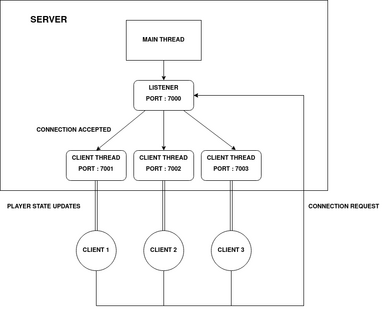
\includegraphics{L1}

\subsection{TCP Server Implementation}
The initial implementation utilized the TCP protocol, chosen for its ease of implementation and built-in features for handling new client connections via port assignments.

\subsubsection{TCP Fallbacks and Challenges}
While TCP was employed in the initial server setup, it proved suboptimal for real-time multiplayer gaming \cite{tcpnotneeded}. The protocol introduced noticeable latency and wait times for clients, attributable to TCP's inherent design for reliable data transmission through packet acknowledgment. Although this ensures data integrity, crucial in many applications, it hampers the speed and responsiveness needed in real-time gaming.

Nevertheless, certain project features were conducive to TCP implementation. Consequently, a hybrid approach was adopted, incorporating UDP for faster communication while integrating a simplified version of TCP's reliability system for specific functionalities.

\subsection{UDP Implementation}
\subsubsection{UDPServer Class}
The UDPServer class is built on the UDP protocol, prioritizing reduced latency over reliability to enhance real-time communication efficiency.

\paragraph{UDP Server Functionality}
    In this implementation, the server retains some TCP functionalities: it waits for client connection requests, assigns unique ports to each client for dedicated communication, and creates new threads for concurrent communication.

\paragraph{Client-Server Communication}
    Communication between the client and server is managed through custom message classes. These classes encode messages into JSON strings for network transmission. The code snippets for these custom classes are as follows:

\begin{lstlisting}[style=pythonstyle]

class PacketClass:
    type = None
    msg = None

    def __init__(self,type=None,msg=None):
    

class LoginResMsg:
    type = None
    msg = None

    def __init__(self,x,y,id):
        
    def getJson(self):
        return json.dumps(self.__dict__)



class JsonPacket:
    type = None
    msg = None
    def __init__(self,type=None,msg=None):
        if type :
            self.type=type
            if self.type!=LOGIN_REQ and self.type != UDP_CON_REQ:
                self.msg=json.loads(msg)
            else:
                self.msg = msg

    def udpConnReq(self):
        self.type = UDP_CON_REQ
        self.msg = None
        return self.getJson()

    def udpConnRes(self,socket):
        self.type = UDP_CON_RES
        self.msg = str(socket)
        return self.getJson()

    def loginReq(self,username):
        self.type=LOGIN_REQ
        self.msg=username
        return self.getJson()

    def loginRes(self,spawn):
        self.type=LOGIN_RES
        self.msg=spawn.getJson()
        return self.getJson()

    def playerUpdate(self,player):
        self.type=PLAYER_UPDATE
        self.msg=player.getJson()
        return self.getJson()

    def gameStateUpdate(self,game_state):
        self.type=GAME_STATE
        self.msg=game_state.getJson()
        return self.getJson()

    def getJson(self):
        return json.dumps(self.__dict__)






class DataPlayer:
    position=[0,0]
    yaw=0
    shoot=False
    health = None
    shotWho=None
    def __init__(self,position=[0,0],yaw=0,shoot=False,health=None,shotWho=None):
        self.position=position
        self.yaw=yaw
        self.shoot=shoot
        self.health=health
        self.shotWho=shotWho
    def update(self,position=[0,0],yaw=0,shoot=False):
        self.position=position
        self.yaw=yaw
        self.shoot=shoot
    def show(self):
        print(self.__dict__)
    def __str__(self):
        return str(self.__dict__)
    def getJson(self):
        # print(self.__dict__)
        return json.dumps(self.__dict__)

    \end{lstlisting}

\subsection{Game State Management}
The game state is dynamically updated based on data received from each client. In this architecture, the server primarily functions as a communication medium, with the game logic being executed client-side. To illustrate this concept, consider an example involving two players, Player A and Player B. When Player A shoots Player B, the client-side code of Player A recognizes this action and updates the server. Subsequently, the server informs Player B's client to adjust its health accordingly.

\subsubsection{Game State Class Functions}
The Game State Class encompasses several key functions:

\begin{itemize}
    \item It stores and continuously updates player data.
    \item It provides methods for serializing the game state into JSON format, facilitating efficient network transmission.
    \item It implements specific game logic, such as ray casting algorithms, to determine player visibility and other in-game interactions.
\end{itemize}

The code implementation for these functions is provided below:
\begin{lstlisting}[style=pythonstyle]

    
class Game_State:
    running=False
    players={}
    # score=0
    map_obj=None

    def __init__(self,running=False,players={},map_obj=None):
        self.running=running
        self.players=players
        self.map_obj=map_obj

    def get_players_json(self,id):
        temp={}
        for i , player in self.players.items():
            temp[str(i)]=str(player.__dict__)
        temp[str(-1)]=str(id)
        return json.dumps(temp,indent=1)
        
    def show(self,id =None):
        print("Game State: ###########\n")
        if id:
            for i, player in self.players.items():
                if i != id:
                    print(f"Player {i}: {player}") 
        else:
            for i, player in self.players.items():
                
                print(f"Player {i}: {player}")
        print("############\n\n")
        # for i in self.players:
        # 	i.show()

    def getJson(self):
        return json.dumps(self.players)
        \end{lstlisting}

\subsection{Pseudocode for Server Flow}
\begin{verbatim}
    1. UDPMultiCliCon Class:
    - Create a UDP socket and bind it to a specified address and port.
    - Include methods to:
      - Receive data from clients.
      - Accept login requests and allocate spawn positions.
      - Update the game state and send it to clients.
 
 2. UDPServerCon Class:
    - Create a UDP socket for the main server connection.
    - Include methods to:
      - Accept incoming messages.
      - Send connection information to clients (like assigned ports).
 
 3. UDPServer Class:
    - Initialize game state and a dictionary to manage client handlers.
    - Assign new ports for clients to maintain separate communication channels.
    - In the `start` method:
      - Continuously listen for new connections.
      - For each new connection, assign a port and start a new thread for handling the client.
      - Send the client their unique communication port.
    - In the `handle_client` method:
      - Manage communication with individual clients.
      - Update the game state based on client actions.
      - Handle client disconnections and remove them from the game state.
 
 4. Main Server Execution:
    - Define the server host and port.
    - Create an instance of the UDPServer class.
    - Call the `start` method on the server instance to begin listening for and handling client connections.
\end{verbatim}

\subsection{Client-Side Implementation}
The client-side architecture of the project is centered around a primary class, referred to as the Main Connection Class, which is responsible for managing communication with the server. This class utilizes the previously mentioned message classes to format data for transmission. Key functionalities include:

\begin{itemize}
    \item Establishing and maintaining a stable connection with the server.
    \item Encoding and decoding data using custom message classes.
    \item Handling real-time data transmission to ensure synchronized gameplay.
\end{itemize}

Detailed code for the Main Connection Class and its associated functionalities will be provided in the final section of this document.
\begin{lstlisting}[style=pythonstyle]

    class UDPCon:
        s=None
        sendMsg=None
        revMsg=None
        cliAddr = None
        port = None
        host=HOST
        def __init__(self,host=None,port=None):
            self.s = socket.socket(socket.AF_INET, socket.SOCK_DGRAM)
            self.s.settimeout(0.5)
            if host:
                self.host=host
        def accMsg(self):
            self.revMsg , self.cliAddr = self.s.recvfrom(RECIEVE_BUFFER_SIZE)
            self.revMsg = json.loads(self.revMsg)
            print("DATA REC "+self.recvMsg["type"],self.recvMsg["msg"])
            self.recvMsg=JsonPacket(self.recvMsg["type"],self.recvMsg["msg"])
            if self.recvMsg.type != UDP_CON_REQ:
                return None,None
            return self.recvMsg,self.cliAddr
    
        def sendConnMsg(self):
            self.sendMsg=JsonPacket()
            self.sendMsg=self.sendMsg.udpConnReq()
            sent =False
            while not sent:
                try:
                    self.s.sendto(self.sendMsg.encode("utf-8"), (self.host,PORT))
                    self.revMsg = self.s.recvfrom(RECIEVE_BUFFER_SIZE)[0]
                    sent = True
                except Exception as e:
    
                    print(e)
                    sent = False
                    continue
            self.revMsg = json.loads(self.revMsg)
            print("DATA REC "+self.revMsg["type"],self.revMsg["msg"])
            return int(self.revMsg["msg"])
            # return 7001
    
        def login(self,username):
            
            print(self.host,self.port)
    
            self.sendMsg=JsonPacket()
            self.sendMsg=self.sendMsg.loginReq(username)
            sent = False
            while not sent:
                try:
            # sleep(0.5)
                    self.s.sendto(self.sendMsg.encode("utf-8"), (self.host,self.port))
                # except timeout of socket
                    
            
                    self.revMsg = self.s.recvfrom(RECIEVE_BUFFER_SIZE)[0]
                    sent = True
                except Exception as e:
                    print(e)
                    sent = False
    
    
            print(self.revMsg)
            self.revMsg = json.loads(self.revMsg)
            self.revMsg=JsonPacket(self.revMsg["type"],self.revMsg["msg"])
            # print([int(self.revMsg.msg['x']),int(self.revMsg.msg['y']),int(self.revMsg.msg['id'])])
            return [int(self.revMsg.msg["x"]),int(self.revMsg.msg["y"]),int(self.revMsg.msg["id"])]
            
        def playerUpdate(self,player):
            self.sendMsg=JsonPacket()
            self.sendMsg=self.sendMsg.playerUpdate(player)
    
            sent = False
            while not sent:
                try:
    
                    self.s.sendto(self.sendMsg.encode("utf-8"),(self.host,self.port))
                    self.revMsg = self.s.recvfrom(RECIEVE_BUFFER_SIZE)[0]
                    sent = True
                except Exception as e:
                    print(e)
                    sent = False
                    continue
            
    
    
            print(self.revMsg)
            self.revMsg = json.loads(self.revMsg)
            self.revMsg = JsonPacket(self.revMsg["type"], self.revMsg["msg"])
            return self.revMsg
\end{lstlisting}

The client is initialized and connected to the server by sending a formatted connection message. The initial connection setup is as follows:

\begin{lstlisting}[style=pythonstyle]
connector = UDPCon(host=host)
porttemp = connector.sendConnMsg()
\end{lstlisting}

Once connected, the player logs into the game to receive their initial spawn location and ID, as detailed in the UDPCon class:

\begin{lstlisting}[style=pythonstyle]
spawn_location = connector.login(username)
\end{lstlisting}

Subsequently, during each game cycle, the playerUpdate method in the connector is invoked, and player updates are sent to the server:

\begin{lstlisting}[style=pythonstyle]
obj = DataPlayer([self.player.pos], self.player.angle, self.player.shot, self.player.health, self.player.shotWho)
game_state_res = self.connector.playerUpdate(obj)
\end{lstlisting}

The player update includes the following data:
\begin{itemize}
    \item New position
    \item New angle
    \item Shooting status (whether the player has shot or not)
    \item Health of the player
    \item ID of the player who has been shot, if applicable
\end{itemize}

This process ensures real-time synchronization of player actions and states between the client and the server.

\subsection{Server Finder}
\label{subsec:serverfinder}

The Server Finder is an integral part of the system, as discussed in Section \ref{sec:communication flow}. This tool bridges the gap between starting the server and establishing a connection with it. The Server Finder operates on the local network using the UDP protocol to discover the server. It broadcasts a message on a predefined port, which is consistent across all clients.

A parallel UDP communication system runs alongside the main server on the designated server PC. This system listens for broadcast messages on the specified port. Upon receiving a broadcast, the script responds with the main server's IP address and port number, thus facilitating the client's connection to the server.

The process involves these steps:
\begin{itemize}
    \item Broadcasting a UDP message across the local network.
    \item Listening for these broadcasts on the server-side via a dedicated UDP script.
    \item Responding to the client with the server's IP address and port number.
\end{itemize}

The Server Finder utilizes network scanning tools, such as the `nmap` command, to identify active interfaces on the local network, enabling the effective location of the server. This approach ensures a seamless and automated process for clients to connect to the server within the local network.

\begin{lstlisting}[style=pythonstyle]

def find_all_ips():
    hostname = socket.gethostname()
    IPAddr = socket.gethostbyname(hostname)


    print("Your Computer Name is:" + hostname)
    print("Your Computer IP Address is:" + IPAddr)
    secs=IPAddr.split(".")
    netId= ""
    for i in range(len(secs)-1):
        netId+= secs[i]+"."
    netId+="0"
    print(netId)

    os.system("nmap -n -sn "+netId+"/24 -oG - | awk '/Up$/{print $2}' > ips.txt")
\end{lstlisting}

Continuing with the Server Finder process, the system utilizes the previously identified active IP addresses on the local network. These addresses are used to broadcast a server-finding message. The sequence of actions is as follows:

\begin{itemize}
    \item The system broadcasts a Server Finder message to the stored IP addresses on the local network.
    \item The server, upon receiving this message, is programmed to respond with a specific acknowledgment.
    \item If the response matches the expected format, the IP address and port of the server are then captured and stored by the client.
\end{itemize}

This mechanism ensures that clients within the network can automatically detect and connect to the server without manual input of the server's IP address and port. The process not only streamlines the connection setup but also adds a layer of dynamic interaction in network environments where server details might change or multiple servers might be present.

\begin{lstlisting}[style=pythonstyle]

def find_server():
    file1 = open('ips.txt', 'r')
    Lines = file1.readlines()

    count = 0

    s = socket.socket(socket.AF_INET, socket.SOCK_DGRAM)
    s.settimeout(FINDER_TIMEOUT)
    line =None
    # Strips the newline character
    for line in Lines:
        try:
        # print("-"+line[:-1]+"-")
            s.sendto("server?".encode("utf-8"), (line[:-1],SERVER_FINDER_PORT))
            revMsg , cliAddr = s.recvfrom(RECIEVE_BUFFER_SIZE)
            if revMsg:
                print("request -> "+line+ "\nresponse -> " +revMsg.decode())
                break
            # os.system("ping "+line+" "+str(SERVER_FINDER_PORT))
            count += 1
        except Exception as e:
            print(e)
            continue
    if line:
        return line[:-1]
    else:
        return HOST
\end{lstlisting}


\section{Results}
\label{chap:results}
The final implementation of the multiplayer first-person shooter game showcases a robust network architecture, capable of handling real-time communications with minimal latency. The game state synchronization across clients was successfully achieved, allowing for a seamless multiplayer experience. Key findings include the efficacy of the hybrid TCP/UDP implementation and the dynamic server discovery mechanism, both of which significantly enhanced the game's performance and usability.

\section{Discussion}
\label{chap:discussion}
The results demonstrate a successful balance between reliable data transmission and low-latency communication, crucial for real-time multiplayer gaming. The implementation of a concurrent server with game state management validated the project's approach to handling multiple client interactions simultaneously. The effectiveness of the Server Finder tool in simplifying network connectivity also stands out as a significant achievement.

\subsection{Limitations and Challenges}
Given more time, further optimization of the client-server data exchange could be explored to enhance game performance under various network conditions. One challenge faced was balancing the trade-off between the reliability of TCP and the speed of UDP, particularly in maintaining game state consistency across clients.


\section{Conclusion}
\label{chap:conclusion}
This project has yielded valuable insights into the design and implementation of network systems for multiplayer games. The key achievements include the development of an efficient game state synchronization mechanism and a user-friendly server discovery process. However, further investigations into optimizing network traffic and exploring alternative data transmission methods could provide additional improvements.

\section{Reflections on own work}
\label{chap:reflection}
\begin{itemize}
    \item The scope of the project was refined to focus primarily on network implementation, driven by the challenges in real-time multiplayer gaming.
    \item Extensive research into network protocols and multiplayer game architectures guided the project's direction.
    \item Implementing, testing, and validating the results were informed by a combination of academic research and practical examples in the gaming industry.
    \item Sources like technical forums, networking textbooks, and multiplayer gaming case studies were instrumental in overcoming technical challenges.
    \item Starting over, more emphasis would be placed on early-stage testing of network protocols to better understand their impact on gameplay.
    \item In retrospect, exploring more advanced server discovery mechanisms could have further enhanced the project.
\end{itemize}



\section{source code}


\begin{lstlisting}[style=pythonstyle, caption=msg classes code]
    from settings import *
    import json
    
    
    
    
    class PacketClass:
        type = None
        msg = None
        def __init__(self,type=None,msg=None):
            self.type=type
            self.msg=msg
    
    class LoginResMsg:
        x=0
        y=0
        id=None
        def __init__(self,x,y,id):
            self.x=x
            self.y=y
            self.id=id
        def getJson(self):
            return json.dumps(self.__dict__)
    
    class JsonPacket:
        type=None
        msg=None
        def __init__(self,type=None,msg=None):
            if type :
                # self.type=type
                # self.msg=msg
                self.type=type
            # if msg:
                if self.type!=LOGIN_REQ and self.type != UDP_CON_REQ:
                    self.msg=json.loads(msg)
                    # print(self.msg)
                else:
                    self.msg = msg
        def udpConnReq(self):
            self.type = UDP_CON_REQ
            self.msg = None
            return self.getJson()
        def udpConnRes(self,socket):
            self.type = UDP_CON_RES
            self.msg = str(socket)
            return self.getJson()
        def loginReq(self,username):
            self.type=LOGIN_REQ
            self.msg=username
            return self.getJson()
        def loginRes(self,spawn):
            self.type=LOGIN_RES
            self.msg=spawn.getJson()
            return self.getJson()
        def playerUpdate(self,player):
            self.type=PLAYER_UPDATE
            self.msg=player.getJson()
            return self.getJson()
        def gameStateUpdate(self,game_state):
            self.type=GAME_STATE
            self.msg=game_state.getJson()
            return self.getJson()
        def getJson(self):
            # print(json.dumps(self.__dict__))
            return json.dumps(self.__dict__)
    
        
    
    
    class DataPlayer:
        position=[0,0]
        yaw=0
        shoot=False
        health = None
        shotWho=None
        def __init__(self,position=[0,0],yaw=0,shoot=False,health=None,shotWho=None):
            self.position=position
            self.yaw=yaw
            self.shoot=shoot
            self.health=health
            self.shotWho=shotWho
        def update(self,position=[0,0],yaw=0,shoot=False):
            self.position=position
            self.yaw=yaw
            self.shoot=shoot
        def show(self):
            print(self.__dict__)
        def __str__(self):
            return str(self.__dict__)
        def getJson(self):
            # print(self.__dict__)
            return json.dumps(self.__dict__)
    
    
    
    \end{lstlisting}
    \begin{lstlisting}[style=pythonstyle, caption=server game state class]

class Game_State:
running=False
players={}
# score=0
map_obj=None

def __init__(self,running=False,players={},map_obj=None):
    self.running=running
    self.players=players
    self.map_obj=map_obj
def get_players_json(self,id):
    temp={}
    for i , player in self.players.items():
        temp[str(i)]=str(player.__dict__)
    temp[str(-1)]=str(id)
    return json.dumps(temp,indent=1)
    

def show(self,id =None):
    print("Game State: ###########\n")
    if id:
        for i, player in self.players.items():
            if i != id:
                print(f"Player {i}: {player}") 
    else:
        for i, player in self.players.items():
            
            print(f"Player {i}: {player}")
    print("############\n\n")
    # for i in self.players:
    # 	i.show()
def getJson(self):
    return json.dumps(self.players)
        \end{lstlisting}

        \begin{lstlisting}[style=pythonstyle, caption=server code UDP]
            import os
import sys
print(os.getcwd())
sys.path.insert(0, os.getcwd())
import socket
import json
from render_handels.map import *
from multiprocessing import Process, Manager, Lock
from multiprocessing.managers import BaseManager
from connection_handels.server_classes import *
from server_finder import *
import random
import pickle
from settings import * 

import socket
import threading


class UDPMultiCliCon:
    s=None
    sendMsg=None
    recvMsg=None
    cliAddr=None
    # gameState=None
    playerId=None
    host=HOST
    restricted_area = {(i, j) for i in range(10) for j in range(10)}
    def __init__(self,port=None,host=None,i=None,addr = None):
        self.s = socket.socket(socket.AF_INET, socket.SOCK_DGRAM)
        self.s.settimeout(5.0)
        self.cliAddr = addr
        if host:
            self.host = host
        if port:
            print("present",(self.host,port))
            self.s.bind((self.host,port))
        else:
            self.s.bind((self.host, PORT))
        self.playerId=i
    def recieve(self):
        print("data trying")
        data = self.s.recvfrom(RECIEVE_BUFFER_SIZE)[0]
        print("data recieved ")
        self.recvMsg = json.loads(data)
        # print("DATA REC "+self.recvMsg["type"],self.recvMsg["msg"])
        self.recvMsg=JsonPacket(self.recvMsg["type"],self.recvMsg["msg"])
        return self.recvMsg
    def loginAccepted(self,map_obj):
        print("login acc in")
        self.sendMsg=JsonPacket()
        # x_spawn=random.randrange(1,map_obj.rows-1,1)
        # y_spawn=random.randrange(1,map_obj.cols-1,1)
        pos = x, y = random.randrange(map_obj.cols), random.randrange(map_obj.rows)
        while (pos in map_obj.world_map) or (pos in self.restricted_area):
            pos = x, y = random.randrange(map_obj.cols), random.randrange(map_obj.rows)
        # x_spawn=1
        # y_spawn=2
        # print(x_spawn,y_spawn)
        res= LoginResMsg(x,y,self.playerId)
        self.sendMsg=self.sendMsg.loginRes(res)
        print("login in sending "+self.sendMsg)
        self.s.sendto(self.sendMsg.encode("utf-8"),self.cliAddr)

        return
    def playerUpdate(self,game_state):
        self.sendMsg=JsonPacket()
        self.sendMsg=self.sendMsg.gameStateUpdate(game_state)
        self.s.sendto(self.sendMsg.encode("utf-8"),self.cliAddr)

        return


class UDPServerCon:
    s=None
    sendMsg=None
    recvMsg=None
    cliAddr = None
    host = None
    def __init__(self,port=None,host=None):
        self.s = socket.socket(socket.AF_INET, socket.SOCK_DGRAM)
        if host:
            self.host = host
        if port:
            self.s.bind((self.host,port))
        else:
            self.s.bind((self.host, PORT))
    def accMsg(self):
        self.recvMsg , self.cliAddr = self.s.recvfrom(RECIEVE_BUFFER_SIZE)
        self.recvMsg = json.loads(self.recvMsg)
        print("DATA REC "+self.recvMsg["type"],self.recvMsg["msg"])
        self.recvMsg=JsonPacket(self.recvMsg["type"],self.recvMsg["msg"])
        if self.recvMsg.type != UDP_CON_REQ:
            return None,None
        return self.recvMsg,self.cliAddr

    def sendConnMsg(self,cliPort):
        self.sendMsg=JsonPacket()
        self.sendMsg=self.sendMsg.udpConnRes(cliPort)
        self.s.sendto(self.sendMsg.encode("utf-8"), self.cliAddr)



class UDPServer:
    i=0
    map_obj=Map(None)
    map_obj.get_map()
    game_state=Game_State(map_obj=map_obj)
    i=0
    def __init__(self):
        self.client_handlers = {}
        self.main_connector = UDPServerCon(host=my_ip())
        self.next_available_port = PORT + 1
    def assignPort(self):
        client_port = self.next_available_port
        self.next_available_port += 1
        return client_port

    def start(self):
        print("UDP Server started. Waiting for clients...")
        while True:
            data, addr = self.main_connector.accMsg()

            if data:
                # Assign a new port for this client
                com_port = self.assignPort()
                
                # Start a new thread for this client
                client_thread = threading.Thread(target=self.handle_client, args=(addr, com_port,self.i))
                self.client_handlers[addr] = [client_thread,com_port]
                client_thread.start()
                
                # Inform the client about their unique port
                self.main_connector.sendConnMsg(com_port)
                self.i +=1        

    def handle_client(self, client_addr, com_port,i):
        # Create a new socket for this client
        print(f"Handling client {client_addr} {com_port}")
        print(my_ip())
        connector = UDPMultiCliCon(com_port,my_ip(),i,client_addr)
        

        while True:
            self.game_state.show()

            try:
                recv =connector.recieve()
                # print(recv)
                # print("something")
                if not recv:  # connection is closed by client
                    print(f"Connection closed by {addr}")
                    connector.s.close()
                    del self.game_state.players[i]
                    break
                if recv.type == LOGIN_REQ:
                    connector.loginAccepted(self.map_obj)
                    print(recv.msg + " has joined the game")
                elif recv.type == PLAYER_UPDATE:
                    # print("-------",str(com_port),recv.msg,"-------")
                    if i in self.game_state.players:
                        self.game_state.players[i]["position"] = recv.msg["position"]
                        self.game_state.players[i]["yaw"] = recv.msg["yaw"]
                        self.game_state.players[i]["shoot"] = recv.msg["shoot"]
                        if int(recv.msg["health"]) == int(self.game_state.players[i]["health"])+1:
                            self.game_state.players[i]["health"] = recv.msg["health"]
                    else:
                        self.game_state.players[i] = recv.msg

                            
                        # self.game_state.players[i] = recv.msg
                    hurtPlayerId= recv.msg["shotWho"]
                    if hurtPlayerId != None:
                        print("SHOT "+str(hurtPlayerId))
                        print("init health : "+str(self.game_state.players[int(hurtPlayerId)]["health"]))
                        self.game_state.players[int(hurtPlayerId)]["health"]=int(self.game_state.players[int(hurtPlayerId)]["health"])-WEAPON_DAMAGE
                        self.game_state.players[i]["shotWho"]=None
                        print(self.game_state.players[int(hurtPlayerId)]["health"])
                    # print(recv.msg)
                    connector.playerUpdate(self.game_state)
            except Exception as e:
                print("exception : "+str(e))
                connector.s.close()
                if i in self.game_state.players:
                    del self.game_state.players[i]
                break
            # Process data


udp_server = UDPServer()
udp_server.start()




        \end{lstlisting}

        \begin{lstlisting}[style=pythonstyle, caption=client communication classes]

class UDPCon:
    s=None
    sendMsg=None
    revMsg=None
    cliAddr = None
    port = None
    host=HOST
    def __init__(self,host=None,port=None):
        self.s = socket.socket(socket.AF_INET, socket.SOCK_DGRAM)
        self.s.settimeout(0.5)
        if host:
            self.host=host
    def accMsg(self):
        self.revMsg , self.cliAddr = self.s.recvfrom(RECIEVE_BUFFER_SIZE)
        self.revMsg = json.loads(self.revMsg)
        print("DATA REC "+self.recvMsg["type"],self.recvMsg["msg"])
        self.recvMsg=JsonPacket(self.recvMsg["type"],self.recvMsg["msg"])
        if self.recvMsg.type != UDP_CON_REQ:
            return None,None
        return self.recvMsg,self.cliAddr

    def sendConnMsg(self):
        self.sendMsg=JsonPacket()
        self.sendMsg=self.sendMsg.udpConnReq()
        sent =False
        while not sent:
            try:
                self.s.sendto(self.sendMsg.encode("utf-8"), (self.host,PORT))
                self.revMsg = self.s.recvfrom(RECIEVE_BUFFER_SIZE)[0]
                sent = True
            except Exception as e:

                print(e)
                sent = False
                continue
        self.revMsg = json.loads(self.revMsg)
        print("DATA REC "+self.revMsg["type"],self.revMsg["msg"])
        return int(self.revMsg["msg"])
        # return 7001
    def login(self,username):
        
        print(self.host,self.port)

        self.sendMsg=JsonPacket()
        self.sendMsg=self.sendMsg.loginReq(username)
        sent = False
        while not sent:
            try:
        # sleep(0.5)
                self.s.sendto(self.sendMsg.encode("utf-8"), (self.host,self.port))
            # except timeout of socket
                
        
                self.revMsg = self.s.recvfrom(RECIEVE_BUFFER_SIZE)[0]
                sent = True
            except Exception as e:
                print(e)
                sent = False


        print(self.revMsg)
        self.revMsg = json.loads(self.revMsg)
        self.revMsg=JsonPacket(self.revMsg["type"],self.revMsg["msg"])
        # print([int(self.revMsg.msg['x']),int(self.revMsg.msg['y']),int(self.revMsg.msg['id'])])
        return [int(self.revMsg.msg["x"]),int(self.revMsg.msg["y"]),int(self.revMsg.msg["id"])]
    def playerUpdate(self,player):
        self.sendMsg=JsonPacket()
        self.sendMsg=self.sendMsg.playerUpdate(player)

        sent = False
        while not sent:
            try:

                self.s.sendto(self.sendMsg.encode("utf-8"),(self.host,self.port))
                self.revMsg = self.s.recvfrom(RECIEVE_BUFFER_SIZE)[0]
                sent = True
            except Exception as e:
                print(e)
                sent = False
                continue
        


        print(self.revMsg)
        self.revMsg = json.loads(self.revMsg)
        self.revMsg = JsonPacket(self.revMsg["type"], self.revMsg["msg"])
        return self.revMsg


class ClientCon:
    s=None
    sendMsg = None
    revMsg = None
    def __init__(self):
        self.s = socket.socket()
        self.s.connect((HOST, PORT))
    def login(self):
        self.sendMsg=PacketClass(type=LOGIN_REQ)
        self.sendMsg = pickle.dumps(self.sendMsg)
        self.s.send(self.sendMsg)
        self.revMsg = self.s.recv(RECIEVE_BUFFER_SIZE)
        self.revMsg = pickle.loads(self.revMsg)
        return [self.revMsg.msg.x,self.revMsg.msg.y,self.revMsg.msg.id]
    def playerUpdate(self,obj):
        self.sendMsg=PacketClass(type=PLAYER_UPDATE)
        self.sendMsg.msg = obj
        self.sendMsg = pickle.dumps(self.sendMsg)
        self.s.send(self.sendMsg)
        self.revMsg = self.s.recv(RECIEVE_BUFFER_SIZE)
        self.revMsg = pickle.loads(self.revMsg)
        return self.revMsg.msg

class ClientJsonCon:
    s=None
    sendMsg = None
    revMsg = None
    def __init__(self):
        self.s = socket.socket()
        self.s.connect((HOST, PORT))
    def login(self,username):
        self.sendMsg=JsonPacket()
        self.sendMsg=self.sendMsg.loginReq(username)
        self.s.send(self.sendMsg.encode("utf-8"))

        self.revMsg = self.s.recv(RECIEVE_BUFFER_SIZE)
        self.revMsg = json.loads(self.revMsg)
        self.revMsg=JsonPacket(self.revMsg["type"],self.revMsg["msg"])
        # print([int(self.revMsg.msg['x']),int(self.revMsg.msg['y']),int(self.revMsg.msg['id'])])
        return [int(self.revMsg.msg["x"]),int(self.revMsg.msg["y"]),int(self.revMsg.msg["id"])]
    def playerUpdate(self,player):
        self.sendMsg=JsonPacket()
        self.sendMsg=self.sendMsg.playerUpdate(player)
        self.s.send(self.sendMsg.encode("utf-8"))

        self.revMsg = self.s.recv(RECIEVE_BUFFER_SIZE)
        # print(self.revMsg)
        self.revMsg = json.loads(self.revMsg)
        self.revMsg = JsonPacket(self.revMsg["type"], self.revMsg["msg"])
        return self.revMsg

        

        \end{lstlisting}
        \begin{lstlisting}[style=pythonstyle, caption=client code]
            if __name__ == '__main__':
    # init_new_game()
    username=(LoginState().run())
    find_all_ips()
    host = find_server()
    print(username,host)
    connector = UDPCon(host=host)
    porttemp = connector.sendConnMsg()
    print(porttemp)
    connector.port= porttemp
    spawn_location= connector.login(username)
    # spawn_location= connector.login(username)

    print("---Connected to server---")

    # spawn_location = connector.login()
    
    # spawn_location = connector.login(username)
    # global playerId 
    playerId= spawn_location[2]
    print("spawn location: ",spawn_location)
    game = Game(connector,spawn_location[0],spawn_location[1])
    # game = Game(1,1)

    game.run()



----- updation code  ---------
    obj=DataPlayer([self.player.pos],self.player.angle,self.player.shot,self.player.health,self.player.shotWho)
    
        game_state_res=self.connector.playerUpdate(obj)
            \end{lstlisting}
            \begin{lstlisting}[style=pythonstyle, caption=server finder]
                import os
                from settings import *
                import socket
                # Using readlines()
                
                def my_ip():
                    hostname = socket.gethostname()
                    IPAddr = socket.gethostbyname(hostname)
                    print(IPAddr)
                    return IPAddr
                
                def find_all_ips():
                    hostname = socket.gethostname()
                    IPAddr = socket.gethostbyname(hostname)
                
                    
                    print("Your Computer Name is:" + hostname)
                    print("Your Computer IP Address is:" + IPAddr)
                    secs=IPAddr.split(".")
                    netId= ""
                    for i in range(len(secs)-1):
                        netId+= secs[i]+"."
                    netId+="0"
                    print(netId)
                    
                    os.system("nmap -n -sn "+netId+"/24 -oG - | awk '/Up$/{print $2}' > ips.txt")
                    # os.system("nmap -n -sn 172.16.59.0/24 -oG - | awk '/Up$/{print $2}' ")
                
                
                def find_server():
                    file1 = open('ips.txt', 'r')
                    Lines = file1.readlines()
                    
                    count = 0
                
                    s = socket.socket(socket.AF_INET, socket.SOCK_DGRAM)
                    s.settimeout(FINDER_TIMEOUT)
                    line =None
                    # Strips the newline character
                    for line in Lines:
                        try:
                        # print("-"+line[:-1]+"-")
                            s.sendto("server?".encode("utf-8"), (line[:-1],SERVER_FINDER_PORT))
                            revMsg , cliAddr = s.recvfrom(RECIEVE_BUFFER_SIZE)
                            if revMsg:
                                print("request -> "+line+ "\nresponse -> " +revMsg.decode())
                                break
                            # os.system("ping "+line+" "+str(SERVER_FINDER_PORT))
                            count += 1
                        except Exception as e:
                            print(e)
                            continue
                    if line:
                        return line[:-1]
                    else:
                        return HOST
                
            \end{lstlisting}
            \begin{lstlisting}[style=pythonstyle, caption=server assigner]
                import socket
                import string
                from settings import *
                hostname = socket.gethostname()
                IPAddr = socket.gethostbyname(hostname)
                
                 
                print("Your Computer Name is:" + hostname)
                print("Your Computer IP Address is:" + IPAddr)
                
                s = socket.socket(socket.AF_INET, socket.SOCK_DGRAM)
                s.bind((IPAddr,SERVER_FINDER_PORT))
                while(True):
                    recvMsg , cliAddr = s.recvfrom(RECIEVE_BUFFER_SIZE)
                
                    if recvMsg.decode() == "server?":
                        print("req")
                
                        s.sendto("yes".encode("utf-8"), cliAddr)
                
                \end{lstlisting}

        \newpage

Further work on this project could involve the integration of WebSockets to enable internet-based gameplay, expanding the game's reach beyond local networks. This would involve tackling additional challenges related to broader network variability and security considerations.